\chapter{Многогранные углы}\label{ch:ch5}

\begingroup
\setlength{\intextsep}{10pt plus 2pt minus 2pt}
\setlength{\textfloatsep}{12pt plus 2pt minus 2pt}

% А. П. Киселёв, «Элементарная геометрия», 23-е издание, 1914. Печатные с. 300–306.
% Страницы скана планиметрии на 11 больше печатных.
\newcommand*{\kiselevPlanimetryPage}[2]{%
    \href{https://commons.wikimedia.org/wiki/File:\%D0\%90._\%D0\%9F._\%D0\%9A\%D0\%B8\%D1\%81\%D0\%B5\%D0\%BB\%D1\%91\%D0\%B2._\%D0\%AD\%D0\%BB\%D0\%B5\%D0\%BC\%D0\%B5\%D0\%BD\%D1\%82\%D0\%B0\%D1\%80\%D0\%BD\%D0\%B0\%D1\%8F_\%D0\%B3\%D0\%B5\%D0\%BE\%D0\%BC\%D0\%B5\%D1\%82\%D1\%80\%D0\%B8\%D1\%8F_(1914).djvu?page=#1}{#2}%
}

% Печатная с. 300.
\kiselevparagraph{para:polyhedral-angle-definition} \textbf{Определение.} Возьмём несколько углов (рис.~\ref{fig:kiselev-stereo-343}): \(ASB\), \(BSC\), \(CSD\), \(\ldots\), которые, примыкая последовательно друг к другу, расположены в одной плоскости вокруг общей вершины \(S\).

\begin{figure}[htbp]
    \centering
    \renewcommand{\thefigure}{343}
    \captionsetup{name=Рис.,labelsep=period}
    \begin{tikzpicture}[line cap=round,line join=round]
    \coordinate (S) at (0,0);
    \draw[thick] (S) -- (-2.94,2.41) node[above left] {\(A\)}
        (S) -- (-3.58,-0.25) node[left] {\(B\)}
        (S) -- (-1.96,-2.84) node[below left] {\(C\)}
        (S) -- (0.27,-3.29) node[below] {\(D\)}
        (S) -- (2.24,-2.76) node[below right] {\(E\)}
        (S) -- (2.69,2.57) node[above right] {\(F\)};
    \node[above] at (S) {\(S\)};
\end{tikzpicture}

    \caption{Плоские углы вокруг общей вершины \(S\)}\label{fig:kiselev-stereo-343}
\end{figure}

Повернём плоскость угла \(ASB\) вокруг общей стороны \(SB\) так, чтобы эта плоскость образовала некоторый двугранный угол с плоскостью \(BSC\). Затем, сохраняя получившийся двугранный угол, повернём его вокруг прямой
% Печатная с. 301.
\(SC\) так, чтобы плоскость \(BSC\) образовала некоторый двугранный угол с плоскостью \(CSD\). Продолжим такое последовательное вращение вокруг каждой общей стороны. Если при этом последняя сторона \(SF\) совместится с первой стороной \(SA\), то образуется фигура (рис.~\ref{fig:kiselev-stereo-344}), которая вместе с частью пространства, ограниченной плоскостями, называется \emph{многогранным углом}.

\begin{figure}[htbp]
    \centering
    \renewcommand{\thefigure}{344}
    \captionsetup{name=Рис.,labelsep=period}
    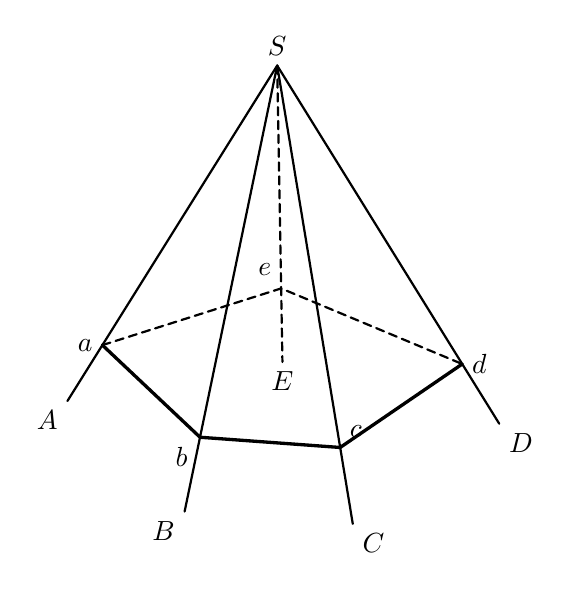
\begin{tikzpicture}[line cap=round,line join=round]
    \coordinate (S) at (0,3.33);
    \coordinate (a) at (-2.22,-0.22);
    \coordinate (b) at (-0.98,-1.39);
    \coordinate (c) at (0.80,-1.52);
    \coordinate (d) at (2.35,-0.46);
    \coordinate (e) at (0.05,0.50);

    \foreach \vertex/\tip in {a/A,b/B,c/C,d/D}{
        \path (S) -- (\vertex) coordinate[pos=1.20] (\tip);
        \draw[thick] (S) -- (\tip);
    }
    \path (S) -- (e) coordinate[pos=1.33] (E);
    \draw[thick,densely dashed] (S) -- (E) (a) -- (e) -- (d);
    \draw[very thick] (a) -- (b) -- (c) -- (d);
    \node[above] at (S) {\(S\)};
    \node[left] at (a) {\(a\)};
    \node[below left,xshift=-1pt] at (b) {\(b\)};
    \node[above right] at (c) {\(c\)};
    \node[right] at (d) {\(d\)};
    \node[above left,yshift=1pt] at (e) {\(e\)};
    \node[below left] at (A) {\(A\)};
    \node[below left] at (B) {\(B\)};
    \node[below right] at (C) {\(C\)};
    \node[below right] at (D) {\(D\)};
    \node[below] at (E) {\(E\)};
\end{tikzpicture}

    \caption{Выпуклый многогранный угол \(SABCDE\)}\label{fig:kiselev-stereo-344}
\end{figure}

Углы \(ASB,BSC,\ldots\) называются \emph{плоскими углами}, или \emph{гранями}, их стороны \(SA,SB,\ldots\) называются \emph{рёбрами}, а общая вершина \(S\) --- \emph{вершиной} многогранного угла. Каждому ребру соответствует свой двугранный угол. Поэтому в многогранном угле столько двугранных углов и столько плоских, сколько в нём всего рёбер. Наименьшее число граней в многогранном угле --- три. Такой угол называется \emph{трёхгранным}. Могут быть углы четырёхгранные, пятигранные и т.~д.

Многогранный угол (рис.~\ref{fig:kiselev-stereo-344}) обозначается или одной буквой \(S\), поставленной у вершины, или рядом букв \(SABCDE\), из которых первая обозначает вершину, а остальные --- рёбра по порядку их расположения.

Многогранный угол называется \emph{выпуклым}, если он весь расположен по одну сторону от каждой своей грани. Таков, например, угол, изображённый на рис.~\ref{fig:kiselev-stereo-344}. Наоборот, угол на рис.~\ref{fig:kiselev-stereo-345} нельзя назвать выпуклым, так как он расположен по обе стороны от грани \(ASB\) или от грани \(BSC\).

\begin{figure}[htbp]
    \centering
    \renewcommand{\thefigure}{345}
    \captionsetup{name=Рис.,labelsep=period}
    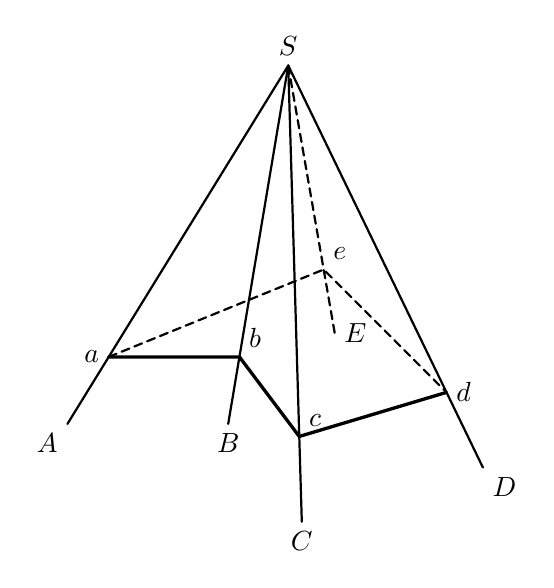
\begin{tikzpicture}[line cap=round,line join=round]
    \coordinate (S) at (0,3.40);
    \coordinate (a) at (-2.28,-0.30);
    \coordinate (b) at (-0.62,-0.30);
    \coordinate (c) at (0.14,-1.31);
    \coordinate (d) at (2.01,-0.75);
    \coordinate (e) at (0.45,0.81);

    \foreach \vertex/\tip in {a/A,b/B,c/C,d/D}{
        \path (S) -- (\vertex) coordinate[pos=1.23] (\tip);
        \draw[thick] (S) -- (\tip);
    }
    \path (S) -- (e) coordinate[pos=1.31] (E);
    \draw[thick,densely dashed] (S) -- (E) (a) -- (e) -- (d);
    \draw[very thick] (a) -- (b) -- (c) -- (d);
    \node[above] at (S) {\(S\)};
    \node[left] at (a) {\(a\)};
    \node[above right] at (b) {\(b\)};
    \node[above right] at (c) {\(c\)};
    \node[right] at (d) {\(d\)};
    \node[above right] at (e) {\(e\)};
    \node[below left] at (A) {\(A\)};
    \node[below] at (B) {\(B\)};
    \node[below] at (C) {\(C\)};
    \node[below right] at (D) {\(D\)};
    \node[right] at (E) {\(E\)};
\end{tikzpicture}

    \caption{Многогранный угол по обе стороны от грани \(ASB\)}\label{fig:kiselev-stereo-345}
\end{figure}

Если две грани\footnote{В издании 1914 года напечатано «две грани». На рис.~\ref{fig:kiselev-stereo-344} и \ref{fig:kiselev-stereo-345} секущая плоскость пересекает все пять граней.} многогранного угла пересечём плоскостью, то в сечении образуется многоугольник \(abcde\) (рис.~\ref{fig:kiselev-stereo-344} и \ref{fig:kiselev-stereo-345}). У выпуклого угла этот многоугольник тоже выпуклый.

Мы будем рассматривать только выпуклые многогранные углы.

\kiselevparagraph{para:trihedral-plane-angle-inequality} \textbf{Теорема. В каждом трёхгранном угле каждый плоский угол меньше суммы двух других плоских углов.}

Очевидно, эта теорема нуждается в доказательстве только в том случае, когда она применяется к плоскому углу,
% Печатная с. 302.
\emph{наибольшему из трёх}. Пусть в угле \(SABC\) (рис.~\ref{fig:kiselev-stereo-346}) наибольший из плоских углов --- \(ASC\). Докажем, что даже этот наибольший угол меньше суммы двух остальных.

\begin{figure}[htbp]
    \centering
    \renewcommand{\thefigure}{346}
    \captionsetup{name=Рис.,labelsep=period}
    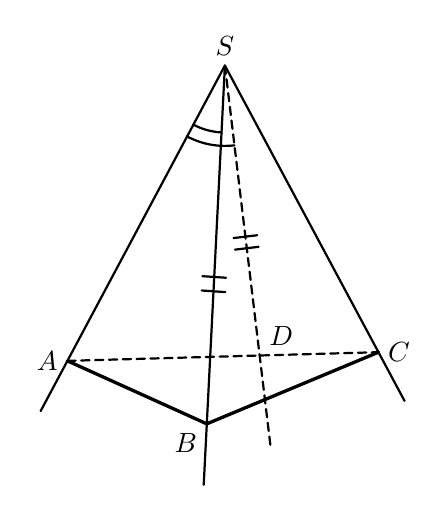
\begin{tikzpicture}[line cap=round,line join=round]
    \coordinate (S) at (0,3.4);
    \coordinate (A) at (-2.00,-0.35);
    \coordinate (B) at (-0.23,-1.15);
    \coordinate (C) at (1.95,-0.24);
    \path (A) -- (C) coordinate[pos=0.618] (D);
    \foreach \point in {A,B,C}{
        \path (S) -- (\point) coordinate[pos=1.17] (tip);
        \draw[thick] (S) -- (tip);
    }
    \path (S) -- (D) coordinate[pos=1.32] (tip);
    \draw[very thick] (A) -- (B) -- (C);
    \draw[thick,densely dashed] (A) -- (C) (S) -- (tip);
    \draw[thick] (S) ++(-118.07:0.85) arc[start angle=-118.07,end angle=-92.90,radius=0.85];
    \draw[thick] (S) ++(-118.07:1.02) arc[start angle=-118.07,end angle=-83.18,radius=1.02];
    \path (S) -- (B) coordinate[pos=0.59] (BmarkA) coordinate[pos=0.63] (BmarkB);
    \path (S) -- (D) coordinate[pos=0.59] (DmarkA) coordinate[pos=0.63] (DmarkB);
    \draw[thick] (BmarkA) ++(-0.15,0.01) -- ++(0.30,-0.02)
        (BmarkB) ++(-0.15,0.01) -- ++(0.30,-0.02)
        (DmarkA) ++(-0.15,-0.018) -- ++(0.30,0.036)
        (DmarkB) ++(-0.15,-0.018) -- ++(0.30,0.036);
    \node[above] at (S) {\(S\)};
    \node[left] at (A) {\(A\)};
    \node[below left] at (B) {\(B\)};
    \node[right] at (C) {\(C\)};
    \node[above right] at (D) {\(D\)};
\end{tikzpicture}

    \caption{Плоские углы трёхгранного угла \(SABC\)}\label{fig:kiselev-stereo-346}
\end{figure}

Отложим на угле \(ASC\) часть \(ASD\), равную \(ASB\). Проведём к плоскости\footnote{В издании 1914 года стоит «к плоскости». На рис.~\ref{fig:kiselev-stereo-346} прямая \(AC\) лежит в плоскости угла \(ASC\).} угла \(ASC\) какую-нибудь прямую \(AC\), пересекающую \(SD\) в некоторой точке \(D\). Отложим \(SB=SD\). Соединив \(B\) с \(A\) и \(C\), получим треугольник \(ACB\), в котором
\[
    AD+DC<AB+BC.
\]

Треугольники \(ASD\) и \(ASB\) равны, так как в каждом из них равный угол заключён между равными сторонами. Следовательно, \(AD=AB\). Поэтому в полученном неравенстве можно отбросить равные части \(AD\) и \(AB\), после чего получим
\[
    DC<BC.
\]

Теперь заметим, что у треугольников \(SCD\) и \(SCB\) две стороны одного равны двум сторонам другого, а третьи стороны не равны. В таком случае против большей из этих сторон лежит больший угол (\kiselevPlanimetryPage{51}{см.~Планиметрия, §~58, пункт~2}). Значит,
\[
    \angle CSD<\angle CSB.
\]

Прибавив к левой части этого неравенства угол \(ASD\), а к правой равный ему угол \(ASB\), получим неравенство, которое требовалось доказать:
\[
    \angle ASC<\angle CSB+\angle ASB.
\]

\textbf{Следствие.} Вычтя из обеих частей последнего неравенства по углу \(ASB\) или по углу \(CSB\), получим\footnote{Обе строки воспроизводят обозначения печатного издания. На рис.~\ref{fig:kiselev-stereo-346} точки \(E\) нет. В предыдущем неравенстве участвуют углы \(ASC\), \(CSB\) и \(ASB\).}:
\[
    \begin{aligned}
        \angle ASC-\angle ASE &< \angle CSB;\\
        \angle ASB-\angle CSE &< \angle ASB.
    \end{aligned}
\]

Так как, кроме того, угол \(ASC\), наибольший из трёх углов, конечно, больше разности двух других углов, то заключаем:

\textbf{В трёхгранном угле каждый плоский угол больше разности двух других углов.}

% Печатная с. 303.
\kiselevparagraph{para:convex-polyhedral-angle-sum} \textbf{Теорема. В каждом выпуклом многогранном угле сумма всех плоских углов меньше} \(4d\)\footnote{Буквой \(d\) обозначен прямой угол.}.

\begin{figure}[htbp]
    \centering
    \renewcommand{\thefigure}{347}
    \captionsetup{name=Рис.,labelsep=period}
    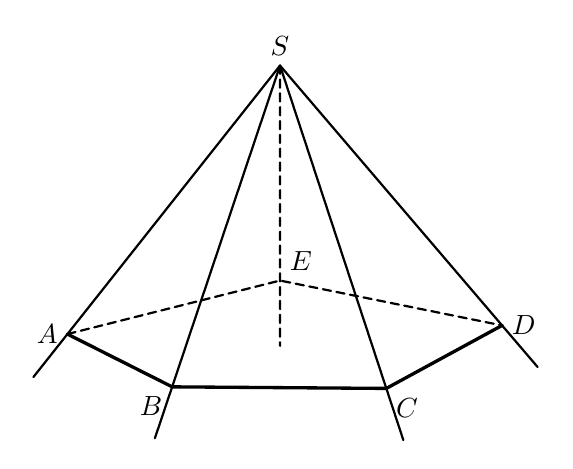
\begin{tikzpicture}[line cap=round,line join=round]
    \coordinate (S) at (0,2.91);
    \coordinate (A) at (-2.70,-0.50);
    \coordinate (B) at (-1.37,-1.17);
    \coordinate (C) at (1.35,-1.19);
    \coordinate (D) at (2.82,-0.39);
    \coordinate (E) at (0,0.18);

    \foreach \point in {A,B,C,D}{
        \path (S) -- (\point) coordinate[pos=1.16] (tip);
        \draw[thick] (S) -- (tip);
    }
    \draw[thick,densely dashed] (S) -- (0,-0.65) (A) -- (E) -- (D);
    \draw[very thick] (A) -- (B) -- (C) -- (D);
    \node[above] at (S) {\(S\)};
    \node[left] at (A) {\(A\)};
    \node[below left] at (B) {\(B\)};
    \node[below right] at (C) {\(C\)};
    \node[right] at (D) {\(D\)};
    \node[above right] at (E) {\(E\)};
\end{tikzpicture}

    \caption{Сечение выпуклого многогранного угла \(SABCDE\)}\label{fig:kiselev-stereo-347}
\end{figure}

Пересечём грани (рис.~\ref{fig:kiselev-stereo-347}) выпуклого угла \(SABCDE\) какой-нибудь плоскостью. В сечении получим выпуклый \(n\)-угольник \(ABCDE\). Применяя \hyperref[para:trihedral-plane-angle-inequality]{теорему предыдущего параграфа} к каждому из трёхгранных углов, образовавшихся при точках \(A\), \(B\), \(C\), \(D\) и \(E\), находим:
\[
    \angle ABC<\angle ABS+\angle SBC;\quad
    \angle BCD<\angle BCS+\angle SCD;\quad \ldots
\]
Сложим почленно все эти неравенства. Тогда в левой части получим сумму всех углов многоугольника \(ABCDE\), которая равна \(2dn-4d\) (\kiselevPlanimetryPage{78}{см.~Планиметрия,~§~89}), а в правой --- сумму углов треугольников \(ASB,BSC,\ldots\), кроме тех углов, которые лежат при вершине \(S\). Обозначив сумму этих последних углов буквой \(x\), получим после сложения:
\[
    2dn-4d<2dn-x.
\]
Откуда
\[
    x<4d.
\]


\section*{Равенство трёхгранных углов}
\addcontentsline{toc}{section}{Равенство трёхгранных углов}

\kiselevparagraph{para:supplementary-trihedral-angle} \textbf{Дополнительный угол.} Из вершины \(S\) (рис.~\ref{fig:kiselev-stereo-348}) трёхгранного угла \(SABC\) проведём к грани \(ASB\) перпендикуляр \(SC_1\), направив его в ту сторону от этой грани, в которой расположено противоположное ребро \(SC\). Подобным образом проведём перпендикуляр \(SA_1\) к грани \(BSC\) и \(SB_1\) к грани \(ASC\). Трёхгранный угол, у которого рёбрами служат полупрямые \(SA_1,SB_1\) и \(SC_1\), называется \emph{дополнительным} для угла \(SABC\).

\begin{figure}[htbp]
    \centering
    \renewcommand{\thefigure}{348}
    \captionsetup{name=Рис.,labelsep=period}
    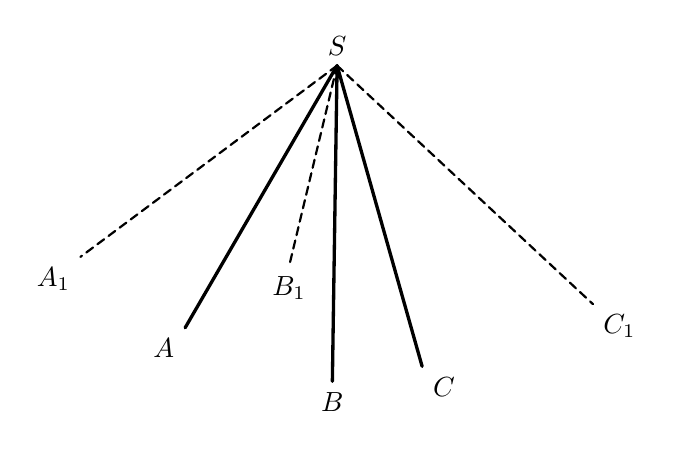
\begin{tikzpicture}[line cap=round,line join=round]
    \coordinate (S) at (0,2.31);
    \draw[very thick] (S) -- (-1.93,-1.02) node[below left] {\(A\)}
        (S) -- (-0.06,-1.70) node[below] {\(B\)}
        (S) -- (1.08,-1.51) node[below right] {\(C\)};
    \draw[thick,densely dashed] (S) -- (-3.26,-0.12) node[below left] {\(A_1\)}
        (S) -- (-0.61,-0.24) node[below] {\(B_1\)}
        (S) -- (3.25,-0.72) node[below right] {\(C_1\)};
    \node[above] at (S) {\(S\)};
\end{tikzpicture}

    \caption{Трёхгранный угол \(SABC\) и дополнительный угол \(SA_1B_1C_1\)}\label{fig:kiselev-stereo-348}
\end{figure}

Заметим, что если для угла \(SABC\) дополнительным углом служит угол \(SA_1B_1C_1\), то и наоборот: для угла \(SA_1B_1C_1\) дополнительным будет \(SABC\). Действительно, плоскость \(SA_1B_1\), проходящая через перпендикуляры к плоскостям \(BSC\) и \(ASC\), перпендикулярна
% Печатная с. 304.
к ним обеим, а следовательно, и к линии их пересечения \(SC\). Значит, прямая \(SC\) перпендикулярна к грани \(SA_1B_1\) и, кроме того, расположена по ту же сторону от этой грани, по которую лежит противоположное ребро \(SC_1\). Подобным образом убедимся, что прямые \(SB\) и \(SA\) соответственно перпендикулярны к граням \(SA_1C_1\) и \(SB_1C_1\) и расположены по ту сторону от них, по которую лежат рёбра \(SB_1\) и \(SA_1\). Значит, углы \(SABC\) и \(SA_1B_1C_1\) \emph{взаимно дополнительны}.

\kiselevparagraph{para:supplementary-trihedral-angle-lemma} \textbf{Лемма 1. Если два трёхгранных угла взаимно дополнительны, то плоские углы одного служат дополнением до} \(2d\) \textbf{к противоположным двугранным углам другого.}

Каждый плоский угол одного из взаимно дополнительных трёхгранных углов образован двумя \emph{перпендикулярами}, проведёнными к граням противоположного двугранного угла другого трёхгранного угла из одной точки его ребра. Заметив это и приняв во внимание направление перпендикуляров, возьмём какой-нибудь двугранный угол \(AB\) (рис.~\ref{fig:kiselev-stereo-349}) и из произвольной точки \(B\) его ребра проведём перпендикуляры: \(BE\) к грани \(AD\) и \(BF\) к грани \(AC\).

\begin{figure}[htbp]
    \centering
    \renewcommand{\thefigure}{349}
    \captionsetup{name=Рис.,labelsep=period}
    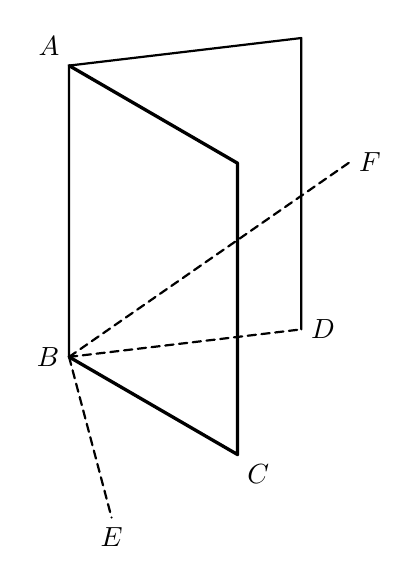
\begin{tikzpicture}[line cap=round,line join=round]
    \coordinate (A) at (0,2.08);
    \coordinate (B) at (0,-1.62);
    \coordinate (C) at (2.14,-2.86);
    \coordinate (D) at (2.95,-1.27);
    \coordinate (E) at (0.54,-3.66);
    \coordinate (F) at (3.56,0.85);

    \draw[thick] (B) -- (A) -- (2.95,2.43) -- (D);
    \draw[very thick] (A) -- (2.14,0.84) -- (C) -- (B);
    \draw[thick,densely dashed] (B) -- (D) (B) -- (E) (B) -- (F);
    \node[above left] at (A) {\(A\)};
    \node[left] at (B) {\(B\)};
    \node[below right] at (C) {\(C\)};
    \node[right] at (D) {\(D\)};
    \node[below] at (E) {\(E\)};
    \node[right] at (F) {\(F\)};
\end{tikzpicture}

    \caption{Перпендикуляры \(BE\) и \(BF\) к граням двугранного угла \(AB\)}\label{fig:kiselev-stereo-349}
\end{figure}

Затем проведём через \(BE\) и \(BF\) плоскость, которая должна быть перпендикулярна к ребру \(AB\) (\hyperref[para:perpendicular-planes-criterion]{см.~§~\ref*{para:perpendicular-planes-criterion}} и \hyperref[para:intersection-normal-to-third-plane]{§~\ref*{para:intersection-normal-to-third-plane}}). Пусть пересечения этой плоскости с гранями угла \(AB\) будут прямые \(BC\) и \(BD\). Тогда угол \(CBD\) должен быть линейным углом двугранного угла \(AB\). Так как стороны угла \(EBF\) соответственно перпендикулярны к сторонам угла \(CBD\) и эти углы не равны, то их сумма равна \(2d\) (\kiselevPlanimetryPage{76}{см.~Планиметрия, §~86}). Это и требовалось доказать.

\kiselevparagraph{para:equal-supplementary-trihedral-angles} \textbf{Лемма 2. Равным трёхгранным углам соответствуют равные дополнительные углы и обратно.}

Равные трёхгранные углы при наложении совмещаются. Поэтому совмещаются и те перпендикуляры, которые образуют рёбра дополнительных углов. Значит, дополнительные углы также совмещаются.

Обратно, если совмещаются дополнительные углы, то совмещаются и данные углы.

\kiselevparagraph{para:trihedral-angle-congruence} \textbf{Теоремы. Трёхгранные углы равны, если они имеют:}

\begin{enumerate}[label=\arabic*),ref=\arabic*]
    \item \textbf{по равному двугранному углу, заключённому между двумя соответственно равными и одинаково расположенными плоскими углами;}
    \item \textbf{или по равному плоскому углу, заключённому между двумя соответственно равными и одинаково расположенными двугранными углами;}
    \item \textbf{или по три соответственно равных и одинаково расположенных плоских угла;}
    \item \textbf{или по три соответственно равных и одинаково расположенных двугранных угла.}
\end{enumerate}

% Печатная с. 305.
\begin{enumerate}[label=\arabic*),ref=\arabic*]
    \item\label{item:trihedral-first-criterion} Пусть \(S\) и \(S_1\) --- два трёхгранных угла (рис.~\ref{fig:kiselev-stereo-350}), у которых
    \[
        \begin{gathered}
            \angle ASB=\angle A_1S_1B_1,\qquad \angle ASC=\angle A_1S_1C_1,\\
            \text{дв. уг. } AS=\text{дв. уг. } A_1S_1.
        \end{gathered}
    \]
    Наложим угол \(S_1\) на угол \(S\) так, чтобы у них совпали точка \(S_1\) с \(S\), прямая \(S_1A_1\) с \(SA\) и плоскость \(A_1S_1B_1\) с \(ASB\). Тогда ребро \(S_1B_1\) пойдёт по \(SB\) (по равенству углов \(A_1S_1B_1\) и \(ASB\)), плоскость \(A_1S_1C_1\) пойдёт по \(ASC\) (по равенству двугранных углов), а ребро \(S_1C_1\) --- по \(SC\) (по равенству углов \(A_1S_1C_1\) и \(ASC\)). Таким образом, трёхгранные углы совместятся всеми своими рёбрами. Значит, они будут равны.

    \begin{figure}[htbp]
        \centering
        \renewcommand{\thefigure}{350}
        \captionsetup{name=Рис.,labelsep=period}
        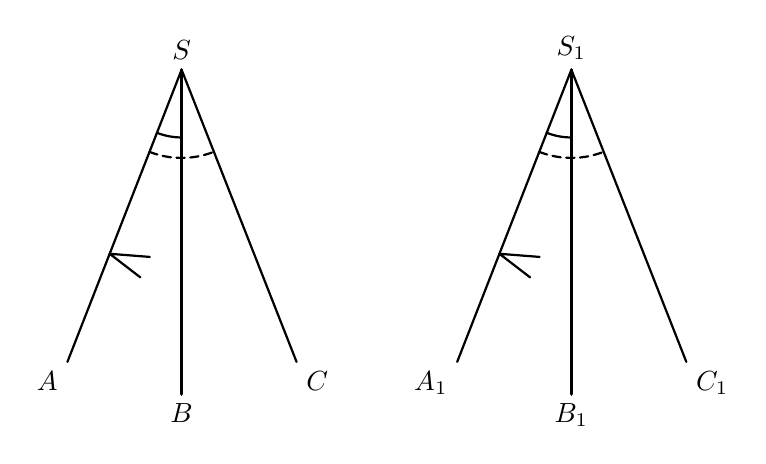
\begin{tikzpicture}[line cap=round,line join=round]
    \foreach \shift/\apex/\lefttag/\fronttag/\righttag in {0/S/A/B/C,4.95/S_1/A_1/B_1/C_1}{
        \begin{scope}[xshift=\shift cm]
            \coordinate (S) at (0,2.27);
            \coordinate (A) at (-1.45,-1.44);
            \coordinate (B) at (0,-1.85);
            \coordinate (C) at (1.46,-1.44);
            \draw[thick] (A) -- (S) -- (C);
            \draw[very thick] (S) -- (B);
            \draw[thick] (S) ++(-111.35:0.86) arc[start angle=-111.35,end angle=-90,radius=0.86];
            \draw[thick,densely dashed] (S) ++(-111.35:1.12)
                arc[start angle=-111.35,end angle=-68.52,radius=1.12];
            \path (S) -- (A) coordinate[pos=0.63] (mark);
            \draw[thick] (mark) -- ++(0.51,-0.04) (mark) -- ++(0.39,-0.30);
            \node[above] at (S) {\(\apex\)};
            \node[below left] at (A) {\(\lefttag\)};
            \node[below] at (B) {\(\fronttag\)};
            \node[below right] at (C) {\(\righttag\)};
        \end{scope}
    }
\end{tikzpicture}

        \caption{Первый признак равенства трёхгранных углов}\label{fig:kiselev-stereo-350}
    \end{figure}

    \item Второй признак доказывается наложением подобно \hyperref[item:trihedral-first-criterion]{первому}.

    \item Пусть \(S\) и \(S_1\) (рис.~\ref{fig:kiselev-stereo-351}) --- два трёхгранных угла, у которых плоские углы одного равны соответственно плоским углам другого и, кроме того, равные углы одинаково расположены.

    \begin{figure}[htbp]
        \centering
        \renewcommand{\thefigure}{351}
        \captionsetup{name=Рис.,labelsep=period}
        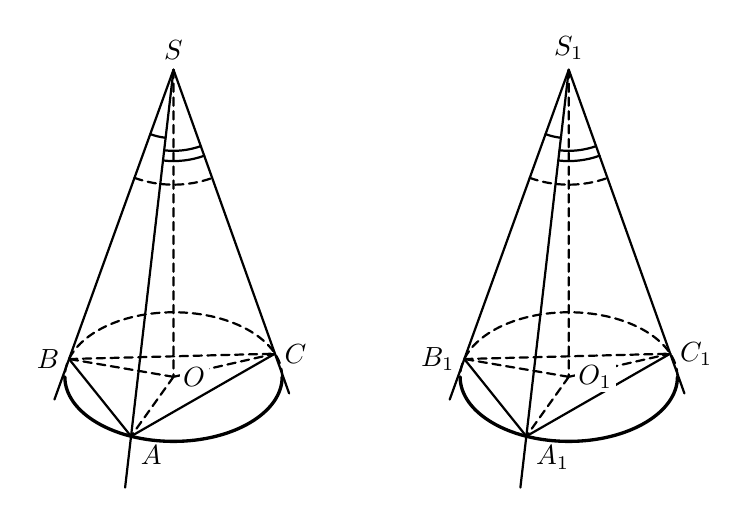
\begin{tikzpicture}[line cap=round,line join=round]
    \foreach \shift/\apex/\fronttag/\lefttag/\righttag/\centre in {0/S/A/B/C/O,5.02/S_1/A_1/B_1/C_1/O_1}{
        \begin{scope}[xshift=\shift cm]
            \coordinate (S) at (0,2.70);
            \coordinate (O) at (0,-1.20);
            \path (O) ++({1.38*cos(247)},{0.82*sin(247)}) coordinate (A);
            \path (O) ++({1.38*cos(164)},{0.82*sin(164)}) coordinate (B);
            \path (O) ++({1.38*cos(21)},{0.82*sin(21)}) coordinate (C);
            \draw[thick,densely dashed] (O) ++(1.38,0)
                arc[start angle=0,end angle=180,x radius=1.38,y radius=0.82];
            \draw[very thick] (O) ++(-1.38,0)
                arc[start angle=180,end angle=360,x radius=1.38,y radius=0.82];
            \draw[thick,densely dashed] (S) -- (O) (O) -- (A) (O) -- (B) (O) -- (C) (B) -- (C);

            \foreach \vertex in {A,B,C}{
                \path (S) -- (\vertex) coordinate[pos=1.14] (tip);
                \draw[thick] (S) -- (tip);
            }
            \draw[thick] (B) -- (A) -- (C);
            \draw[thick] (S) ++(-109.87:0.87) arc[start angle=-109.87,end angle=-96.58,radius=0.87];
            \draw[thick] (S) ++(-96.58:1.03) arc[start angle=-96.58,end angle=-70.30,radius=1.03];
            \draw[thick] (S) ++(-96.58:1.16) arc[start angle=-96.58,end angle=-70.30,radius=1.16];
            \draw[thick,densely dashed] (S) ++(-109.87:1.46)
                arc[start angle=-109.87,end angle=-70.30,radius=1.46];

            \node[above] at (S) {\(\apex\)};
            \node[below right] at (A) {\(\fronttag\)};
            \node[left] at (B) {\(\lefttag\)};
            \node[right] at (C) {\(\righttag\)};
            \node[fill=white,inner sep=1.3pt,right,xshift=2pt] at (O) {\(\centre\)};
        \end{scope}
    }
\end{tikzpicture}

        \caption{Трёхгранные углы с соответственно равными плоскими углами}\label{fig:kiselev-stereo-351}
    \end{figure}

    Отложим на всех рёбрах произвольные, но равные отрезки \(SA=SB=SC=S_1A_1=\ldots\) и построим треугольники \(ABC\) и \(A_1B_1C_1\). Из равенства треугольников \(ABS\) и \(A_1B_1S_1\) находим \(AB=A_1B_1\). Подобно этому из равенства других боковых треугольников выводим \(AC=A_1C_1\) и \(BC=B_1C_1\). Следовательно, \(\triangle ABC=\triangle A_1B_1C_1\). Опустим на плоскости этих треугольников перпендикуляры \(SO\) и \(S_1O_1\). Так как наклонные \(SA,SB\) и \(SC\) равны, то должны быть равны их проекции \(OA,OB\) и \(OC\). Значит, точка \(O\) --- центр окружности, описанной около треугольника \(ABC\). Точно
    % Печатная с. 306.
    так же точка \(O_1\) --- центр окружности, описанной около треугольника \(A_1B_1C_1\). У равных треугольников радиусы описанных окружностей равны. Значит, \(OB=O_1B_1\). Поэтому \(\triangle SBO=\triangle S_1B_1O_1\) (по гипотенузе и катету), и, следовательно, \(OS=O_1S_1\). Наложим теперь фигуру \(S_1A_1B_1C_1\) на фигуру \(SABC\) так, чтобы равные треугольники \(A_1B_1C_1\) и \(ABC\) совместились. Тогда совместятся описанные окружности и, следовательно, их центры \(O_1\) и \(O\). Вследствие этого перпендикуляр \(O_1S_1\) пойдёт по \(OS\), и точка \(S_1\) совпадёт с \(S\). Таким образом, трёхгранные углы совместятся всеми своими рёбрами. Значит, они равны.

    \item Четвёртый признак легко доказывается при помощи дополнительных углов. Если у двух трёхгранных углов соответственно равны и одинаково расположены \emph{двугранные углы}, то у дополнительных углов соответственно равны и одинаково расположены \emph{плоские углы} (\hyperref[para:supplementary-trihedral-angle-lemma]{см.~§~\ref*{para:supplementary-trihedral-angle-lemma}}). Следовательно, дополнительные углы равны. А если равны дополнительные углы, то равны и данные углы (\hyperref[para:equal-supplementary-trihedral-angles]{см.~§~\ref*{para:equal-supplementary-trihedral-angles}}).
\end{enumerate}

\kiselevparagraph{para:symmetric-polyhedral-angles} \textbf{Симметричные многогранные углы.} Как известно, вертикальные углы равны, если речь идёт об углах, образованных прямыми или плоскостями. Посмотрим, применимо ли это к многогранным углам.

Продолжим все рёбра угла \(SABCDE\) за вершину (рис.~\ref{fig:kiselev-stereo-352}). Тогда образуется другой многогранный угол \(SA_1B_1C_1D_1E_1\), который можно назвать \emph{вертикальным} по отношению к первому углу.

\begin{figure}[htbp]
    \centering
    \renewcommand{\thefigure}{352}
    \captionsetup{name=Рис.,labelsep=period}
    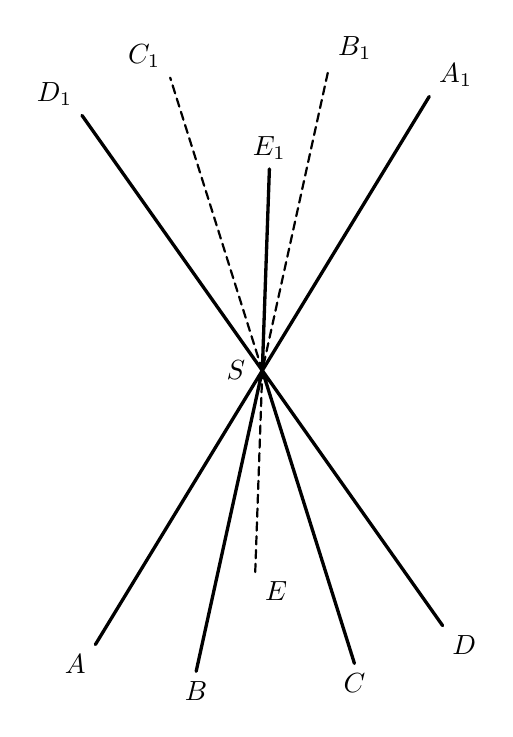
\begin{tikzpicture}[line cap=round,line join=round]
    \coordinate (S) at (0,0);
    \foreach \ray/\x/\y in {A/-2.12/-3.48,B/-0.84/-3.82,C/1.17/-3.72,D/2.29/-3.24,E/-0.09/-2.56}{
        \coordinate (\ray) at (\x,\y);
        \coordinate (\ray-opp) at ({-(\x)},{-(\y)});
    }
    \draw[very thick] (A) -- (A-opp) (B) -- (S) -- (C) (D) -- (D-opp) (S) -- (E-opp);
    \draw[thick,densely dashed] (E) -- (S) -- (B-opp) (S) -- (C-opp);
    \node[left,inner sep=3pt,xshift=-3pt] at (S) {\(S\)};
    \node[below left] at (A) {\(A\)};
    \node[below] at (B) {\(B\)};
    \node[below] at (C) {\(C\)};
    \node[below right] at (D) {\(D\)};
    \node[below right] at (E) {\(E\)};
    \node[above right] at (A-opp) {\(A_1\)};
    \node[above right] at (B-opp) {\(B_1\)};
    \node[above left] at (C-opp) {\(C_1\)};
    \node[above left] at (D-opp) {\(D_1\)};
    \node[above] at (E-opp) {\(E_1\)};
\end{tikzpicture}

    \caption{Симметричные углы \(SABCDE\) и \(SA_1B_1C_1D_1E_1\)}\label{fig:kiselev-stereo-352}
\end{figure}

Нетрудно видеть, что у обоих углов равны соответственно и плоские углы, и двугранные. Но и те и другие расположены \emph{в обратном порядке}. Действительно, если представим наблюдателя, который смотрит изнутри многогранного угла на его вершину, то рёбра \(SA,SB,SC,SD,SE\) будут казаться ему расположенными против движения часовой стрелки. Глядя же на угол \(SA_1B_1C_1D_1E_1\), он увидит рёбра \(SA_1,SB_1,\ldots\) расположенными по движению часовой стрелки.

Многогранные углы с соответственно равными плоскими и двугранными углами, расположенными в обратном порядке, в общем случае не могут совместиться при наложении. Значит, они не равны. Такие углы называются \emph{симметричными} (относительно вершины \(S\)).

\clearpage
\endgroup
